%************************************************
\chapter{Pruebas de Conocimiento Cero}\label{ch:zkp} 
%************************************************

% REF
% Fundamentals
% https://es.wikipedia.org/wiki/Prueba_de_conocimiento_cero
% https://en.wikipedia.org/wiki/Interactive_proof_system
% 


% Intro
% Ejemplo intuitivo del laberinto
% Pruebas interacticas: completitud y solvencia/solidez/robustez == completo y robusto/sólido, apartado corto, poner QR en el siguiente
% Prueba de conocimiento cero
%	Perfect vs Comp.
%	QR: es Perfect ZKP, y aplicaciones (id de Shamir, ...)
%	


% Para la estadística referenciar:
% JL Gomez Pardo Introduction to cryptography with Mapple
% Elementos probabilidad Zoroa
%
% Fundamentals
% https://en.wikipedia.org/wiki/Computational_indistinguishability


% TODO: teorema de que el logaritmo discreto tiene un ZKP (para Schnorr). Buscar si existe demostración, por si no es perfect

%TODO: lista de ventajas de Handbook of applied? pag 408

Las pruebas de conocimiento cero, con siglas ZKP del inglés \textit{Zero-Knowledge Proofs}, permiten demostrar la veracidad de una declaración, sin revelar nada más de ella. En las ZKP intervienen dos partes, el \textit{Prover} y el \textit{Verifier}, o probador y verificador. El prover asegura que una declaración es cierta, y el verifier quiere convencerse de ello a través de una interacción con el prover, de modo que al final de la misma, o bien acaba convencido de que la declaración es cierta, o bien descubre, con una alta probabilidad, que el prover mentía.

Las pruebas de conocimiento cero surgen a partir de los sistemas de pruebas interactivas, que forman una parte importante de la teoría de complejidad computacional, y pidiendo la propiedad de \textit{conocimiento cero} obtenemos el subconjunto de sistemas interactivos que conforman las pruebas de conocimiento cero.

Las referencias para este capítulo se pueden encontrar en %TODO


\section{Una pequeña historia}
%Wikipedia

Antes de estudiar formalmente las ZKP, vamos a ver un ejemplo que se publicó originalmente como un cuento sobre la cueva de Alí Babá \citep{ZKPcave:story}, pero que aquí adaptamos para resumirlo.

\hfil

Imaginemos una cueva donde el camino se bifurca y al final de cada pasillo se juntan ambos caminos formando una especie de anillo. En el punto en que se unen dentro de la cueva, hay una puerta con un código secreto que permite abrirla desde ambos lados, para cruzar al otro pasillo.

\textbf{P}eggy conoce la clave secreta y quiere \textbf{p}robarlo a su amigo Víctor, pero sin tener que revelársela.
\marginpar{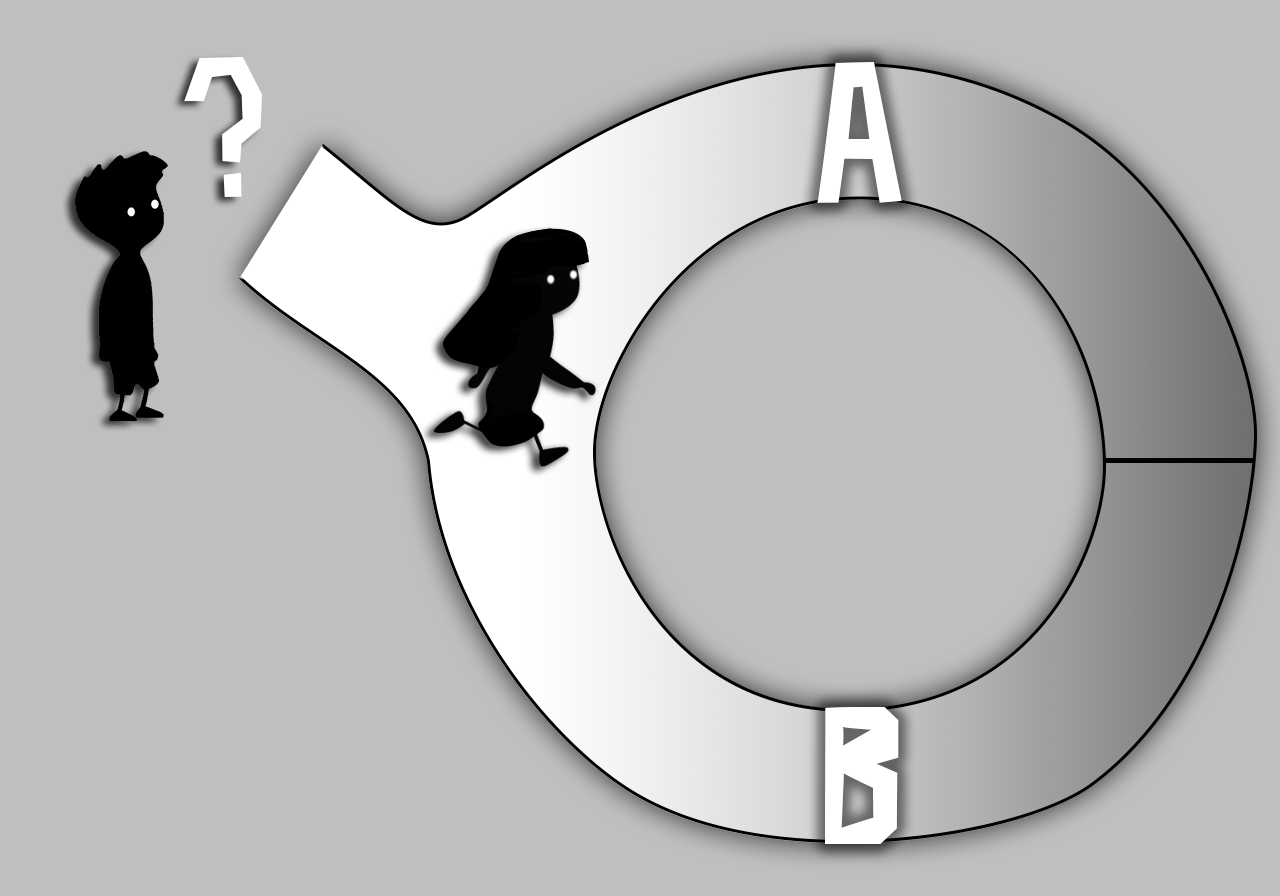
\includegraphics[width=1.\linewidth]{gfx/graficoJL_ZKP_1}\\La cueva \citep{ZKPcave:fig}. Peggy entra por A o B al azar. Víctor espera fuera.}
Peggy y Víctor quedan en la entrada de la cueva con unos \textit{walkie-talkies}, de modo que Víctor esperará fuera y Peggy entrará a la cueva y tomará uno de los pasillos, que llamaremos A y B, sin decirle cuál a Víctor.

%\begin{figure}[bth]
%	\begin{center}
%		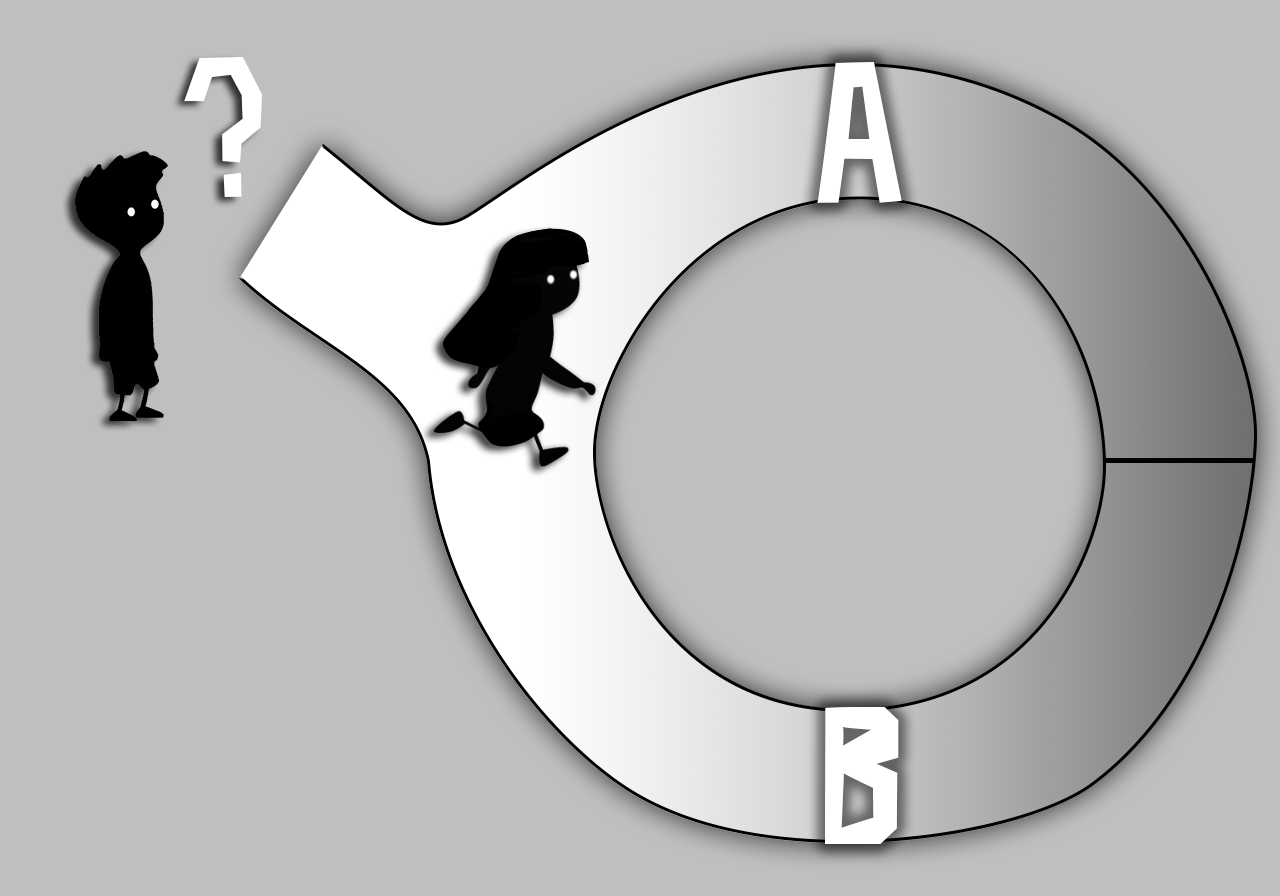
\includegraphics[width=.45\linewidth]{gfx/graficoJL_ZKP_1}
%	\end{center}
%	\caption{La cueva \citep{ZKPcave:fig}. Peggy entra por A o B al azar, Víctor espera fuera.}
%	\label{fig:ZKPcave1}
%\end{figure}

Al llegar a la puerta, avisa a Víctor para que entre a la cueva y espere en la bifurcación, donde \textbf{V}íctor, para intentar \textbf{v}erificar que Peggy conoce la clave, le indicará por qué pasillo quiere que vuelva, el A o el B.


%\begin{figure}[bth]
%	\begin{center}
%		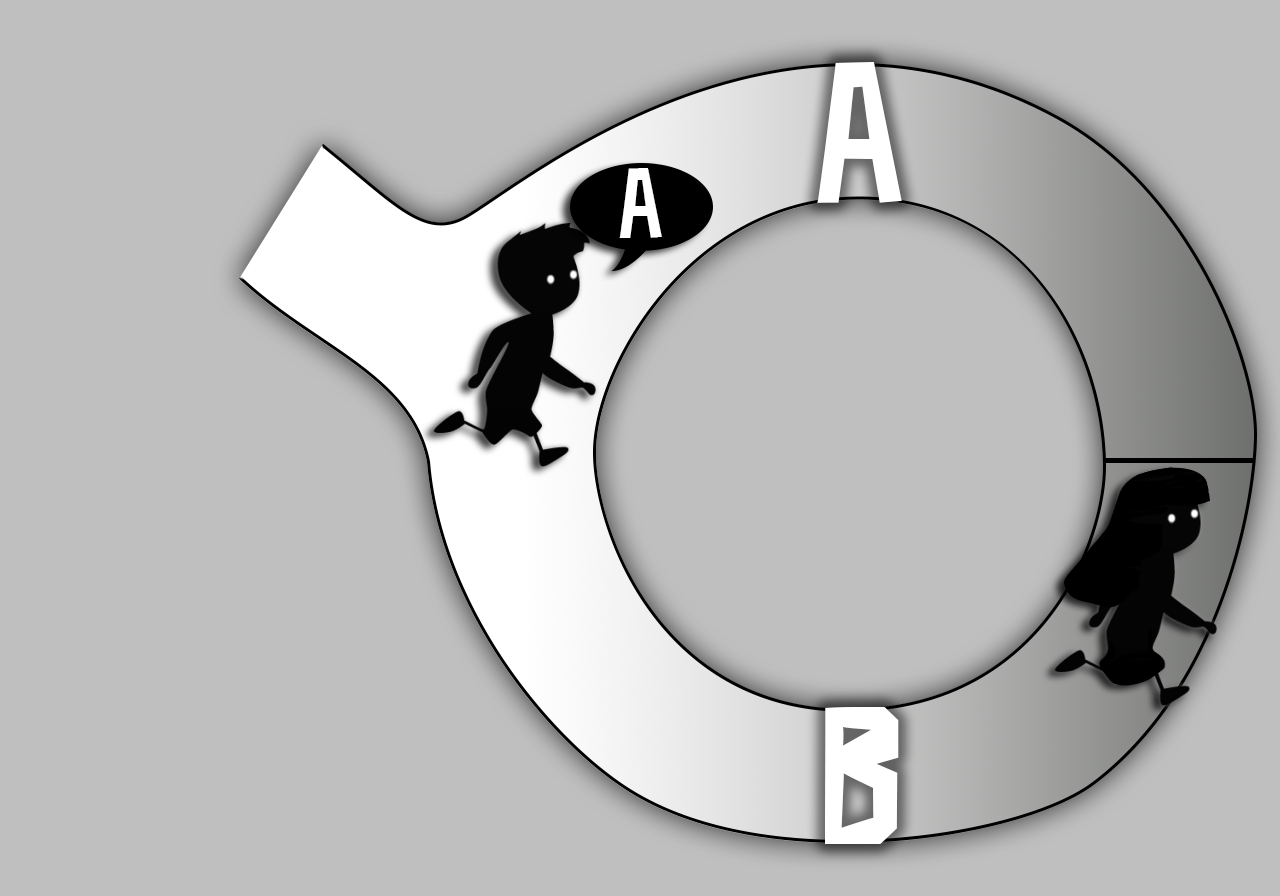
\includegraphics[width=.45\linewidth]{gfx/graficoJL_ZKP_2}
%	\end{center}
%	\caption{La cueva. Víctor elige al azar por dónde quiere que regrese Peggy.}
%	\label{fig:ZKPcave2}
%\end{figure}

Si Peggy realmente conoce la clave, podrá volver a la bifurcación por el pasillo solicitado, abriendo, si es preciso, la puerta.\marginpar{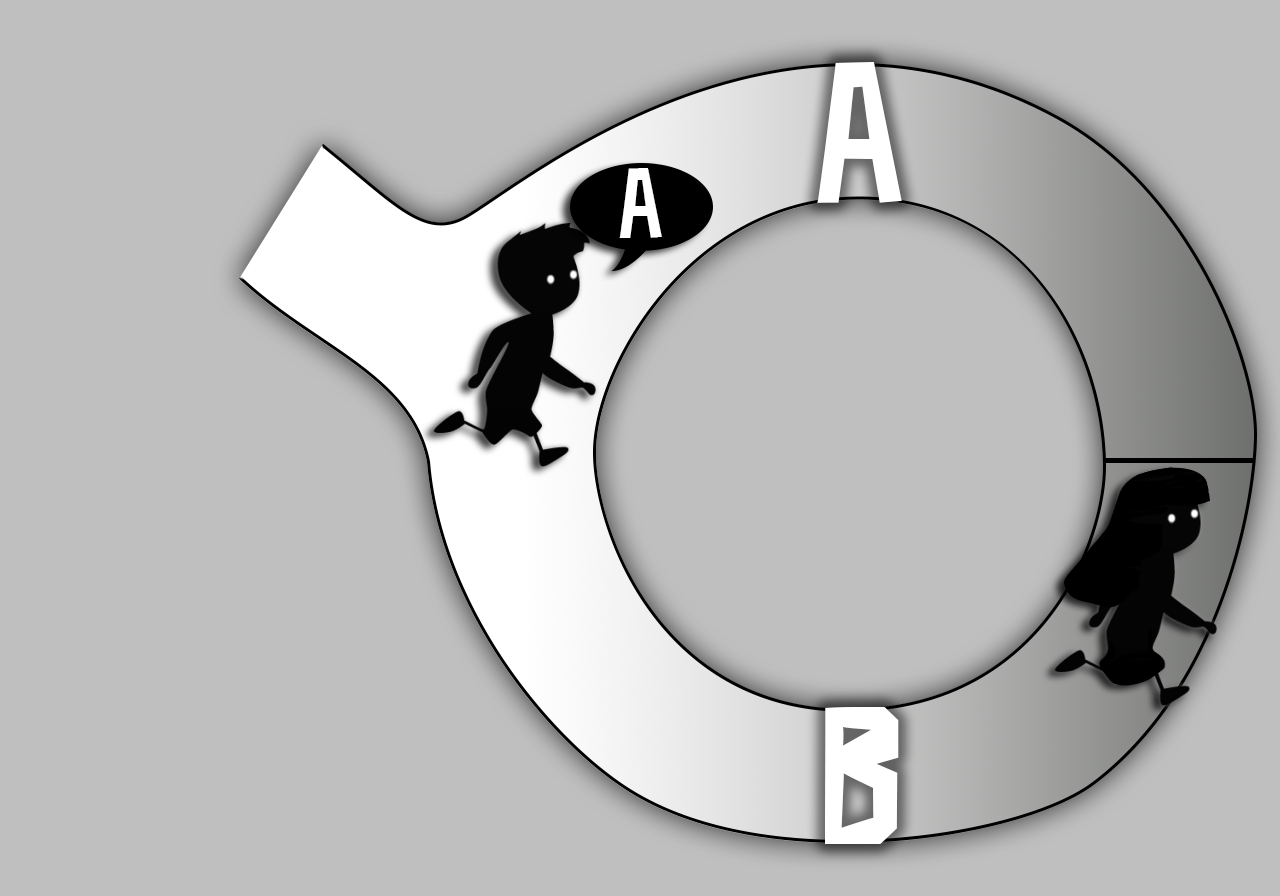
\includegraphics[width=1.\linewidth]{gfx/graficoJL_ZKP_2}\\La cueva. Víctor elige al azar por dónde quiere que regrese Peggy.}
En caso de que no conociera la clave, al entrar tenía una probabilidad del $50\%$ de adivinar qué pasillo pediría Víctor.


%\begin{figure}[bth]
%	\begin{center}
%		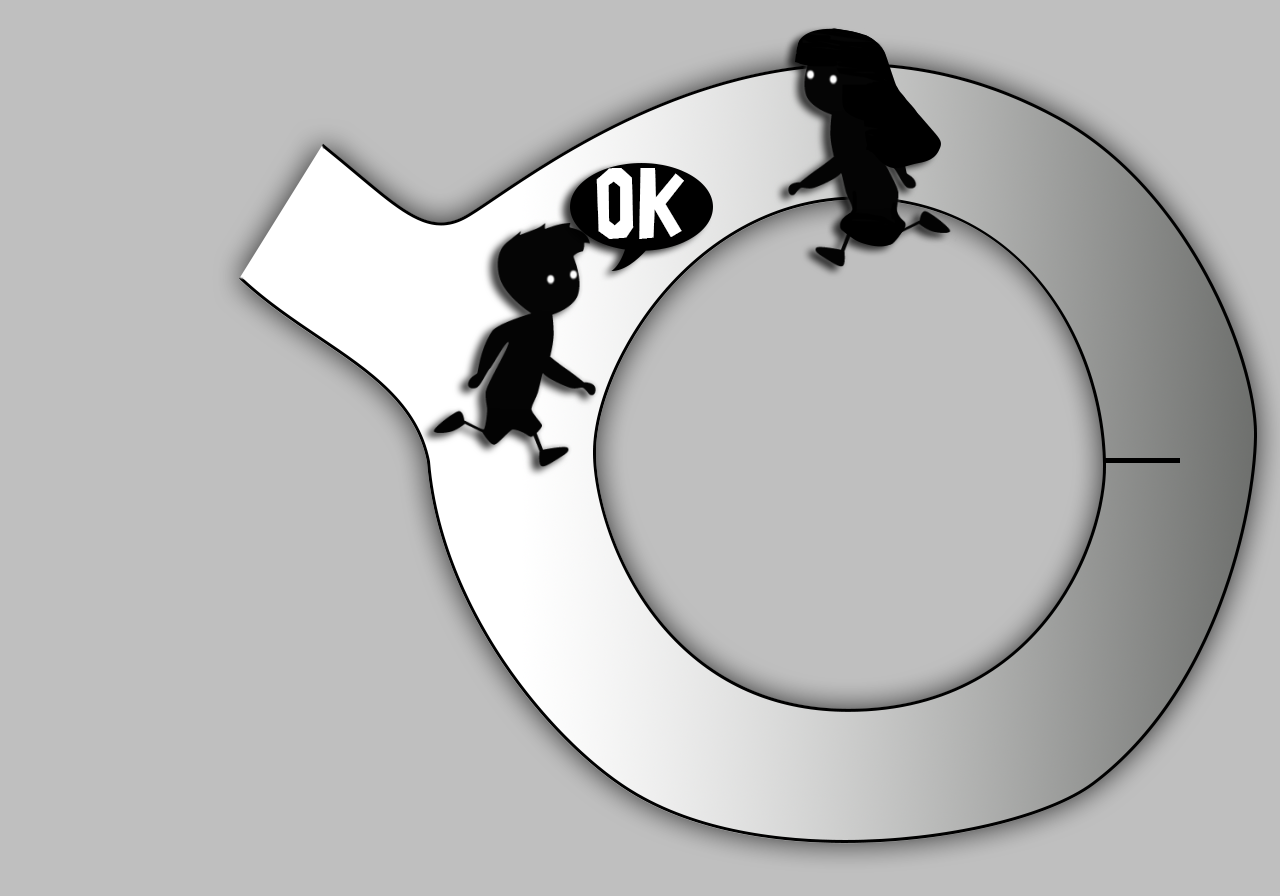
\includegraphics[width=.45\linewidth]{gfx/graficoJL_ZKP_3}
%	\end{center}
%	\caption{La cueva. Peggy vuelve por el camino pedido.}
%	\label{fig:ZKPcave3}
%\end{figure}

Víctor no se queda contento con una sola prueba, así que la repiten hasta que se convence. Si lo repitieran, por ejemplo, 20 veces, Peggy tendría solo una probabilidad de $2^{-20}$, prácticamente nula, de acertar todas las veces y engañar a Víctor.
\marginpar{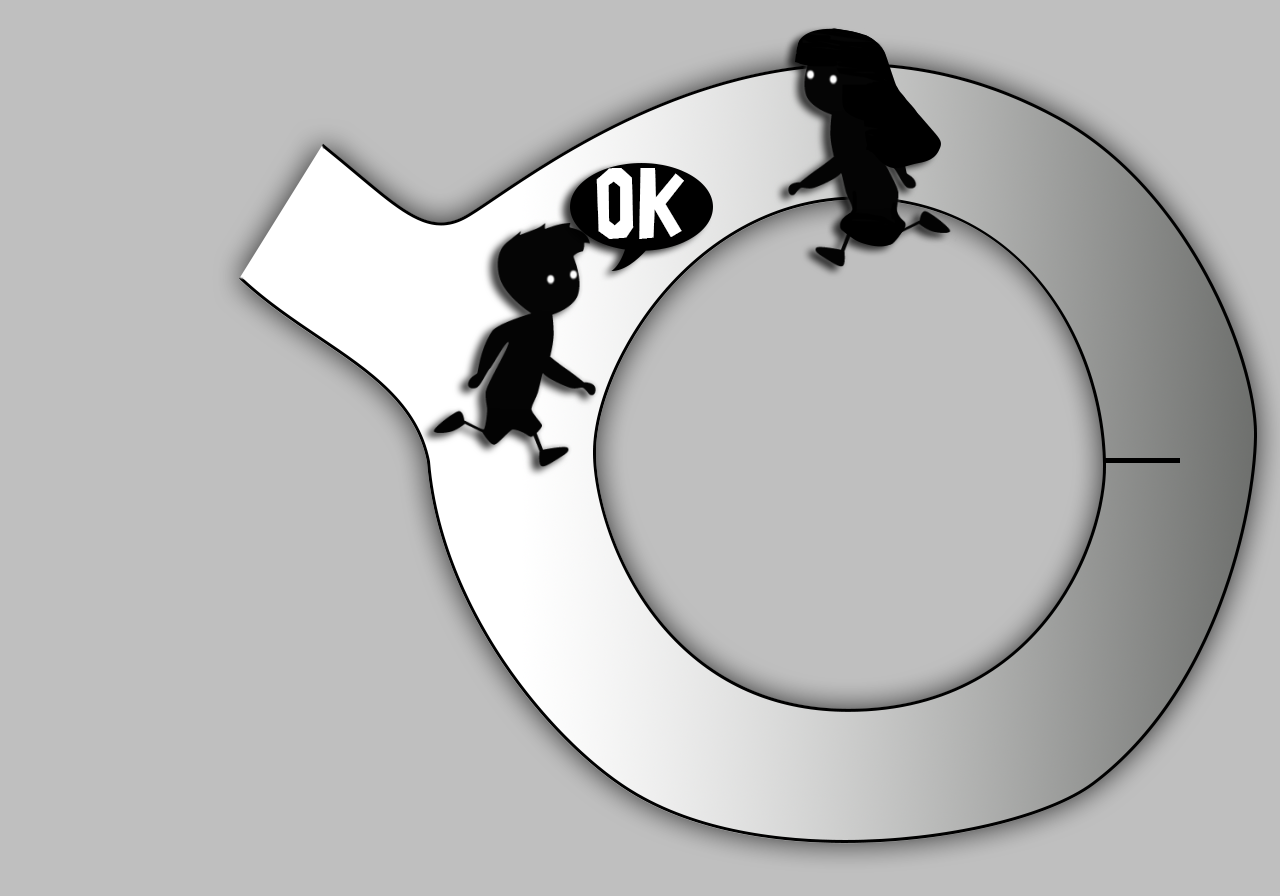
\includegraphics[width=1.\linewidth]{gfx/graficoJL_ZKP_3}\\La cueva. Peggy vuelve por el camino pedido.}


\textbf{E}va, curiosa de qué hacían Víctor y Peggy en la cueva, \textbf{e}spía a Víctor durante todo el proceso. Eva no sabe si Peggy y Víctor han acordado previamente qué pasillo pedir por el \textit{walkie-talkie}, y sólo Víctor está seguro de que los estaba eligiendo al azar.%, por eso, Eva no puede estar segura de si Peggy conoce la clave secreta, o bien estaban \textbf{s}imulando todo para engañarla por cotilla.

Más tarde Eva habla con Víctor, que está seguro de que Peggy conoce la clave, y éste querría convencer también a Eva, pero como él no conoce la clave, no puede repetir la prueba a Eva, sólo Peggy puede realizarla con éxito.

\hfil

\section{Sistemas de Pruebas Interactivas}

Un \textit{sistema de prueba interactivo} es un concepto de la teoría computacional que modela el intercambio de un número finito de mensajes entre dos partes, el probador P y el verificador V, con el objetivo de que P demuestre a V que una instancia de un problema de decisión es $Verdadera$. V tiene una capacidad de cómputo limitada, a lo sumo un algoritmo probabilístico de tiempo de cómputo polinomial. P es computacionalmente todopoderoso. Al final del intercambio de mensajes, o bien V acepta que la instancia es $Verdadera$, o bien la rechaza por ser $Falsa$.

\begin{definition}

	
	Se dice que un problema de decisión $Q$, no necesariamente en \textbf{NP},  tiene un \textit{sistema de prueba interactivo} si tiene un protocolo de interacción polinomialmente acotado en número de mensajes que cumple:
	
	\begin{itemize}
		\item \textit{Completitud} Para toda instancia $q$ $Verdadera$, del problema $Q$, V acepta $q$ como $Verdadera$. 
		\item  \textit{Robustez} Para cada instancia $q$ $Falsa$, ningún P, incluso si no sigue el protocolo, puede convencer a V de que $q$ es $Verdadera$, excepto con una pequeña probabilidad.
		\item Alternativa:
		\item \textit{Robustez} Para cada instancia $q$ $Falsa$, V rechaza la prueba de $q$ con una probabilidad no menor que $\epsilon = 1-n^{-c}$, para cualquier constante $c>0$ y donde $n$ es el tamaño de la instancia.
	\end{itemize}

\end{definition}

En resumen, si la instancia del problema $Q$ que P quiere demostrar es $Verdadera$, el protocolo siempre funciona, no hay falsos negativos, pero si la instancia es $Falsa$, hay una pequeña probabilidad de que $V$ la acepte como $Verdadera$, pueden haber falsos positivos una probabilidad casi despreciable.

Un P o un V que no siguen el protocolo e intentan romper estas propiedades, los llamaremos un P o V \textit{tramposos}.


\begin{definition}
	Denominamos clase de problemas \textbf{IP} (Interactivos en tiempo Polinomial) al conjunto de problemas de decisión para los que existe un sistema de prueba interactivo.
\end{definition}

\begin{proposition}
	\textbf{NP} $\subset$ \textbf{IP}.
\end{proposition}

\begin{proof}
	Sea $Q$ un problema \textbf{NP}. Definimos el siguiente protocolo:

	\begin{enumerate}
		\item  P resuelve la instancia del problema gracias a su capacidad de cómputo ilimitada y genera el certificado para V, que existe para cualquier instancia $Verdadera$ por $Q\in$ \textbf{NP} (\ref{def:NP}).
		\item  V recibe y puede verificar el certificado en tiempo polinomial. Si es válido, V acepta como $Verdadera$ la instancia. Si no, rechaza la prueba.
	\end{enumerate}

	El protocolo es completo y robusto, con probabilidad nula de falso positivo, pues si la instancia es $Falsa$, ningún P, honesto o tramposo, puede generar un certificado que no existe.

\end{proof}


\hfil

\paragraph{Prueba Interactiva para el Problema QR}

\hfil

\hfil

Vamos a ver una prueba interactiva para demostrar que un entero $x$ con Símbolo de Jacobi 1 respecto a $n$, $x \in \mathbb{Z}^Q_n$, es un residuo cuadrático, $x \in \mathbb{Z}^{Q+}_n$.

\hfil

\begin{tabular}{|ll}
	\textit{Nombre:} & Problema QR. \\
	\textit{Parámetros:} &Un entero compuesto impar $N$, y el entero $x\in \mathbb{Z}^Q_N$. \\
	\textit{Pregunta:} & ¿Es $x$ un residuo cuadrático, $x \in \mathbb{Z}^{Q+}_N$? \\
\end{tabular}
\\

\hfil

Una instancia $Verdadera$ del problema es un $x$ residuo cuadrático módulo $N$. Una prueba interactiva para demostrar que $x$ es residuo cuadrático es la siguiente:

\hfil

\rule{\textwidth}{1pt}
\begin{algorithm}[Prueba interactiva para QR]
	
	\hfil
	
	\textit{Datos comunes}: Una instancia ($x$, $N$) del Problema QR. $n$ es el tamaño de la instancia.
	
	\textit{Protocolo}: Sea $t(n)$ un polinomio en $n$. P y V repiten $t(n)$ veces los siguientes pasos.
	
	\begin{enumerate}
		
		\item P $\rightarrow$ V :\quad $u \in_R \mathbb{Z}^{Q+}_N$ \quad (P elige aleatoriamente $u$ en $\mathbb{Z}^{Q+}_N$).
		
		\item V $\rightarrow$ P :\quad $b \in_R \{0,\,1\}$.
		
		\item P $\rightarrow$ V :\; $w$,\; una raíz cuadrada módulo $N$ aleatoria, de $x$ si $b=0$, o bien de $x\cdot u$ si $b=1$.
		
		\item V comprueba si:
		\[
			w^2 \overset{?}{\equiv}
			\begin{cases}
				u\, mod\, N, & si\ b = 0\\
				xu\, mod\, N, & si\ b = 1.\\
			\end{cases}
		\]
		
		Si la comparación falla, V termina en rechazo. En caso contrario, vuelve al paso 1.
		
		
	\end{enumerate}

	Tras $t(n)$ rondas, V termina y acepta la instancia como $Verdadera$, $x$ es un residuo cuadrático módulo $N$.
	
	\label{QRinteractive:alg}
\end{algorithm}
\rule{\textwidth}{1pt}

\hfil


\begin{theorem}
	El problema QR tiene un sistema de prueba interactiva.
	\label{theo:QRint}
\end{theorem}

\begin{proof}
	
	El protocolo se ejecuta $t(n)$ veces, un número de iteraciones polinomialmente asociado al tamaño $n$ de la entrada, por lo que hay un número finito de mensajes que V, computacionalmente limitado, puede llevar a cabo. 
	
	\hfil 
	
	Queda ver que el protocolo anterior es completo y robusto.
	
	La prueba es \textit{completa}, pues para cualquier instancia $Verdadera$ de QR, $x \in \mathbb{Z}^{Q+}_N$, V acepta la prueba de P. En cada iteración, como P es computacionalmente todopoderoso, puede calcular $w$, una raíz cuadrada módulo $N$ de $x$ o $xu$, según el valor de $b$, ambos en $\mathbb{Z}^{Q+}_N$.
	
	Para una instancia $Falsa$, $x \in \mathbb{Z}^{Q-}_N$, cuando V envíe $b=1$, si P sigue el protocolo $u$ será un residuo cuadrático, pero $x\cdot u$ es un no-residuo cuadrático módulo $N$, por lo que no podrá calcular $w$ por mucho poder computacional ilimitado que tenga. Un P tramposo podría intentar engañar a V en el caso $b = 1$ eligiendo $u$ tal que $xu$ es un residuo cuadrático, pero entonces $u$ es un no-residuo cuadrático y fallaría la prueba si $b=0$.
	
	Una vez P se compromete con un $u$, residuo cuadrático o no, la probabilidad de que V lo rechace en esa iteración es $1\/2$, según elija $b=0$ ó $1$. Como el protocolo se ejecuta $t(n)$ veces, la probabilidad de que un P tramposo pueda engañara V en todos es de $2^{-t(n)}$. Vemos entonces que el protocolo cumple la propiedad de \textit{robustez}.
\end{proof}


% TODO: para la presentación, si preguntan por qué t(n) depende del tamaño de la entrada, preparar ejemplo de Z_5 o Z_15 mejor, por 15=3*5 los primos impares, indicar que hay 7 residuos cuadráticos y 7 no-residuos, que la cantidad de u's distintos que puede tomar aleatoriamente de entre los rq y los no-rq para intentar engañarlo es mínima, y en pocas iteraciones pueden haber probado todas las combinaciones, y seguir el protocolo es repetir valores ya contrastados, y comparando con primos de 2048 bits, se pueden pedir más iteraciones.


\section{Pruebas de conocimiento cero}

% Introducción: De manera informal,....
% Definiciones: Prueba de conocimiento (como subconjunto de pruebas de problemas de decisión?), Ensemble, View, Simulator

%TODO: ahora que se habla más de un secreto, que es lo que queremos mantener privado en P, demostrar de la robustez, que si un cheating P no conoce el secreto, pero pasa la prueba, tiene un conocimiento equivalente al secreto. Dem por tema de la probabilidad.


Entre las pruebas interactivas existe un subconjunto que llamamos de \textit{conocimiento cero} si durante el protocolo no se puede inferir información de P, aparte de la veracidad de la instancia. En particular, aún tras realizar la prueba, y estar V convencido, éste no podría repetirla a otro verificador tomando el lugar de P.

\hfil

Antes de ver una definición más formal de una prueba de conocimiento cero, necesitamos algunas definiciones previas.



\begin{definition}
	Llamamos \textit{Vista} a una transcripción de los mensajes intercambiados entre P y V durante la ejecución de una prueba interactiva.
\end{definition}

% Notación de una Vista

Pensemos en un protocolo con 3 mensajes por iteración. En la $i$-ésima ronda, P envía a V el valor $A_i$ como \textit{compromiso}, V responde con el \textit{reto} aleatorio $B_i$, y P termina enviando la \textit{prueba} $C_i$. La tupla $(A_i,\,B_i,\,C_i)$ son variables aleatorias de los posibles valores que se pueden intercambiar en una iteración. La Vista de la prueba interactiva sería $(A_1,\,B_1,\,C_1,\,A_2,\,B_2,\,C_2,\dots ,\,A_{t(n)},\,B_{t(n)},\,C_{t(n)})$, la secuencia de los $t(n)$ mensajes intercambiados entre P y V.

Una Vista sólo es de interés para una instancia $Verdadera$, donde P realmente conoce si es $Verdad$. Para una instancia cuya prueba falla, o bien es realmente una instancia $Falsa$ o P no puede probarla, por ser tramposo y no conocer una prueba o \textit{secreto} que le permita pasar la prueba exitosamente con mayor probabilidad que la de los falsos positivos.


\begin{definition}
	Llamamos ensamble probabilístico, o \textit{ensemble} en inglés, a una familia numerable de variables aleatorias: $\{X_i\}_{i\in I}$, con $I$ numerable.
\end{definition}

Podemos estudiar entonces una Vista como un ensamble probabilístico. Dos Vistas serán iguales cuando las distribuciones de sus variables aleatorias sean idénticas.


\hfil

Denotaremos con V$^*$ a un verificador tramposo. Éste podría no generar los retos $B_i$ anteriores de manera independiente, podría incluso utilizar información previa de otras Vistas para generar los $B_i$ en un intento de extraer información extra de P. A esta información previa la llamaremos $h$ (historial).

Para una instancia $q$ y un verificador cualquiera V$^*$, escribimos la Vista de una prueba como:

\begin{center}
	$Vista_{P,V^*}(q,h) = (q,\,h,\,A_1,\,B_1,\,C_1, \dots ,\,A_{t(n)},\,B_{t(n)},\,C_{t(n)})$.
\end{center}

El verificador tramposo V$^*$ generará los retos $B_i$ con una función probabilística de tiempo polinomial $F$ tal que
\marginpar{Para un verificador honesto $F$ sería un generador de números aleatorios que no utiliza ninguno de los parámetros de entrada.}

\begin{center}
	$B_i = F(q,\,h,\,A_1,\,B_1,\,C_1, \dots ,\,A_{i-1},\,B_{i-1},\,C_{i-1},\,A_i)$.
\end{center}



\begin{definition}
	Un Simulador $S_{V^*}(q,h)$ es un algoritmo probabilístico de tiempo polinomial, que utiliza toda la información que V$^*$ tiene disponible (el historial $h$ y la función $F$), para generar una transcripción de una prueba interactiva, para una instancia $q$ del problema $Q$, sin necesidad de interactuar con P.
\end{definition}

Un Simulador se puede ver como un generador de ensambles probabilísticos, las Vistas de una prueba.


\hfil

Podemos describir, por fin, la tercera propiedad, además de la \textit{completitud} y \textit{robustez}, que debe tener una prueba de conocimiento cero. Se dice también que son ZKP perfectas porque en la práctica se pueden considerar otras definiciones menos restrictivas, las ZKP estadísticas y computacionales.


%\subsection{Pruebas de conocimiento cero perfectas}

\begin{definition}[Propiedad de conocimiento cero]
	\hfil
	
	Un sistema de prueba interactiva (completo y robusto), para un problema de decisión $Q$, es \textit{perfecta de conocimiento cero} si el ensamble $Vista_{P,V}(q,h)$ es idéntico al ensamble generado por un Simulador $S_{V^*}(q,h)$, para cualquier instancia $Verdadera$ $q\in Q$ y cualquier historial $h$.
\end{definition}

%La existencia de un Simulador $S_{V^*}(q,h)$, cuyos ensambles son iguales que los de una Vista generada entre un P y V honestos, implica que de la Vista no se puede obtener ninguna información que V no tuviera ya antes, pues V podía obtener con el Simulador cuantas Vistas quisiera, con el conocimiento que ya tenía.


%%%%
A primera vista, puede parecernos que nada tiene que ver la existencia de tal Simulador con no poder obtener información de P más allá de si la instancia es $Verdadera$. Pero es precisamente el hecho de que cualquier máquina M, que \textbf{no} conoce la solución, ni un certificado para comprobarla (\ref{def:NP}), pueda generar transcripciones del protocolo idénticas a las que podríamos interceptar a un P y V verídicos. Si M no conoce el secreto, de sus simulaciones nada podemos sacar, y por tanto, tampoco de la interacción entre P y V.

%%%%


\hfil

\subsection{Residuos cuadráticos}

Ahora podemos volver al problema QR, que ya vimos en el \autoref{theo:QRint} que su prueba interactiva cumplía \textit{completitud} y \textit{robustez}.

\begin{theorem}
	La prueba interactiva (\ref{QRinteractive:alg}) del problema QR es de conocimiento cero.
\end{theorem}

\begin{proof}
	Sea $(x,N)$ una instancia $Verdadera$ del problema QR, $\exists y\in \mathbb{Z}_N$ tal que $y^2\equiv x \, mod \, N$. En la $i$-ésima ronda tenemos las siguientes variables aleatorias:
	
	\begin{enumerate}
		\item $U_i$, un residuo cuadrático aleatorio enviado por P en el primer mensaje, $u \in_R \mathbb{Z}^{Q+}_N$.
		
		\item $B_i$, un bit aleatorio generado por V, $b \in_R \{0,\,1\}$.
		
		\item $W_i$, una \textit{prueba} de P, $w \in_R \Omega_u$ o bien $w \in_R \Omega_{xu}$, según el valor de $B_i$, es decir, una raíz cuadrada aleatoria módulo $N$ de $u$ o $xu$, donde $\Omega_u$ y $ \Omega_{xu}$ son el conjunto de raíces cuadradas módulo $N$ de $u$ y $xu$, respectivamente.
	\end{enumerate}
	
	\hfil
	
	La Vista de una prueba para un verificador V$^*$ cualquiera es:
	
	\begin{center}
		$Vista_{P,V^*}(x,N,h) = (x,\,N,\,h,\,U_1,\,B_1,\,W_1, \dots ,\,U_{t(n)},\,B_{t(n)},\,W_{t(n)})$.
	\end{center}
	
	
	Para simplificar la notación, escribiremos la variable aleatoria $V_i=(U_1,\,B_1,\,W_1, \dots ,\,U_i,\,B_i,\,W_i)$.
	
	Para un V honesto, todos los $B_i$ son variables aleatorias independientes, uniformes en $\{0,1\}$. Para un V tramposo, la función $F$, probabilística en tiempo polinomial, genera los valores $b_{i+1} = F(x,N,h,v_i,u_{i+1})$, cuando $V_i = v_i$. Unimos el estudio de ambos casos suponiendo, para un V honesto, $F$ como un generador de bits aleatorio, un lanzamiento de moneda.
	
	Ahora que tenemos toda la información accesible a V$^*$ podemos construir un Simulador:
	
	\hfil 
	
	\rule{\textwidth}{1pt}
	
	\textbf{Simulador para el problema QR} $S_{V^*}(x,N,h)$.
	
	\hfil
	
	\textit{Datos}: \quad $(x,N)$, una instancia $Verdadera$ del problema QR; \quad $h$, transcripciones de ejecuciones previas del protocolo; \quad $v_i$, transcripción de la interacción actual ($i$ rondas).
	
	\textit{Ejecución}: Repetir para $i+1 \leq t(n)$:
	
	\begin{enumerate}
		\item Elegir $b_{i+1} \in_R \{0,\,1\}$
		
		\item Elegir $w_{i+1} \in_R \mathbb{Z}^*_N$
		
		\item \textbf{Si} $b_{i+1} = 0$, \textbf{entonces} calcular \qquad $u_{i+1} \equiv w_{i+1}^2 \, mod \,  N$ \\
			  \textbf{Si no}, \qquad \qquad \qquad \qquad \qquad \qquad \: $u_{i+1} \equiv w_{i+1}^2 \cdot x^{-1} \, mod \,  N$
			  
		\item \textbf{Si} $b_{i+1} = F(x,N,h,v_i,u_{i+1})$, \textbf{entonces} añadir la tupla \\ $(u_{i+1},\,b_{i+1},\,w_{i+1})$ a la transcripción. \\
			  \textbf{Si no}, volver al paso 1.
		
		\item $i = i+1$
		
	\end{enumerate}
	
	\rule{\textwidth}{1pt}
	
	\hfill
	
	El Simulador se diferencia del protocolo \ref{QRinteractive:alg} en que, en vez de elegir primero un residuo cuadrático $u_{i+1}$, elige los valores $b_{i+1}$ y $w_{i+1}$ aleatoriamente, y a partir de ellos calcula $u_{i+1}$. Entonces, una vez tiene el $u_{i+1}$ necesario para la función $F$, calcula el bit que V$^*$ hubiera enviado en una interacción real, y comprueba si es el mismo bit $b_{i+1}$ elegido. Aquí es donde vemos que el Simulador es un algoritmo probabilístico en tiempo del tipo Las Vegas (si obtenemos la tupla $i+1$, será una tupla correcta). La probabilidad de que el bit $b_{i+1}$ sea igual que el obtenido de $F$ es de $1/2$. En promedio, el Simulador necesitará dos rondas por cada tupla $(u_{i+1},\,b_{i+1},\,w_{i+1},\,)$, por lo que el tiempo de ejecución esperado es polinomial. 
	
	
	\hfil
	
	Tenemos una prueba interactiva (\ref{QRinteractive:alg}) que genera las vistas:
	
	 \begin{center}
	 	$Vista_{P,V^*}(x,N,h) = (x,N,h,U_1,B_1,W_1,\dots , U_{t(n)}, B_{t(n)}, W_{t(n)})$,
	 \end{center}
	 
	  y un Simulador que genera las transcripciones:
	  
	  \begin{center}
	  	$S_{V^*}(x,N,h)= (x,N,h,U_1^`,B_1^`,W_1^`,\dots , U_{t(n)}^`, B_{t(n)}^`, W_{t(n)}^`)$.
	  \end{center}
	
	Para terminar la demostración, veamos por inducción en $i$ que son iguales, es decir, cumplen la propiedad de \textit{conocimiento cero}.
	
	\hfil
	
	Para el caso $i=0$ ambos ensambles son constantes, $(x,N,h)=(x,N,h)$, tenemos la misma instancia e historial.
	
	\hfil
	
	Suponemos cierto el caso $i-1$, es decir, el ensamble de la Vista:
	
	 \begin{center}
		$Vista_{P,V^*}(x,N,h) = (x,N,h,U_1,B_1,W_1,\dots , U_{i-1}, B_{i-1}, W_{i-1})$,
	\end{center}
	
	es igual al del Simulador:
	
	\begin{center}
		$S_{V^*}(x,N,h)= (x,N,h,U_1^`,B_1^`,W_1^`,\dots , U_{i-1}^`, B_{i-1}^`, W_{i-1}^`)$.
	\end{center}
	
	\hfill

	Siguiendo el protocolo de la prueba interactiva, se generará la siguiente tupla de la Vista, $(U_i, B_i, W_i)$. La variable $U_i$ se elige al inicio aleatoriamente, por lo que es independiente. La v.a. $B_i$ se calcula con $F$, por lo que depende de $U_i$, $V_{i-1}$ y $h$. $W_i$ depende de ambos. La probabilidad de la tupla nos queda:
	
	\begin{flushleft}
		$P(U_i=u, B_i=b, W_i=w) = $ 	$P(U_i=u)\cdot$ \\ 
	 	$ \cdot P(B_i=b \mid V_{i-1}=v, U_i=u,h) \cdot P(W_i=w \mid U_i=u, B_i=b)$
	\end{flushleft}
	
	\hfil
	
	Sea $\alpha = \mid \mathbb{Z}^{Q+}_N \mid $, entonces $P(U_i=u) = \frac{1}{\alpha}$.
	
	Denotamos $ P(B_i=b \mid V_{i-1}=v, U_i=u,h)=p_b$, que dependerá de la $F$ utilizada.
	
	Por último, sea $\beta = \mid \Omega_u \mid = \mid \Omega_{xu} \mid $. Entonces, $P(W_i=w \mid U_i=u, B_i=0) = \frac{1}{\beta}$, $\forall w \in \Omega_u$, y $P(W_i=w \mid U_i=u, B_i=1) = \frac{1}{\beta}$, $\forall w \in \Omega_{xu}$.
	
	En total nos queda, $P(U_i=u, B_i=b, W_i=w) = \frac{p_b}{\alpha \beta}$.
	
	
	
	\hfil
	
	Ahora veamos la tupla generada por el Simulador, $(U_i^`, B_i^`, W_i^`)$. La v.a. $U_i^`$ se calcula a partir de $B_i^`$ y $W_i^`$. La variable $B_i^`$ depende de $U_i^`$, $V_{i-1}$ y $h$ por $F$ en el paso 4. Y la v.a. $W_i^`$ se elige aleatoriamente.
	
	La probabilidad de la tupla es:
	
	\begin{flushleft}
		$P(U_i^`=u, B_i^`=b, W_i^`=w) = $ 	$P(W_i^`=w)\cdot$ \\ 
		$ \cdot P(B_i^`=b \mid V_{i-1}=v, U_i^`=u,h) \cdot P(U_i^`=u \mid W_i^`=w, B_i^`=b)$
	\end{flushleft}
	
	Sabemos que $\mid \mathbb{Z}^*_N \mid = \alpha \cdot \beta $, por lo que $P(W_i^`=w) = \frac{1}{\alpha \beta}$.
	
	La probabilidad
	\marginpar{-$w\in \Omega_u \Leftrightarrow b=0$ \\-$w\in \Omega_{xu} \Leftrightarrow b=1$ \\ -$W_i^`$, $B_i^`$ indep.}
	\begin{align*}
	P(U_i^`=u)  & = P(U_i^`=u, W_i^`\in \Omega_u \cup \Omega_{xu}, B_i^` \in \{0,1\}) = \\
				&= \sum_{w\in \Omega_u} P(U_i^`=u, W_i^`=w, B_i^` = 0) + \\
				& +	\sum_{w\in \Omega_{xu}} P(U_i^`=u, W_i^`=w, B_i^` = 1) = \\
				&= \sum_{w\in \Omega_u} P(W_i^`=w)P(B_i^` = 0) + \sum_{w\in \Omega_{xu}} P(W_i^`=w)P(B_i^` = 1) = \\
				&=\beta \cdot \frac{1}{\alpha \beta} \cdot (P(B_i^`=0) + P(B_i^`=1)) = \\
				&= \frac{1}{\alpha}
	\end{align*}
	
	indica que $U_i^`$ tiene la misma distribución que $U_i$, de modo que, al calcular $b_{i} = F(x,N,h,v_{i-1},u_{i})$, se tiene 
	$P(B_i^`=b \mid V_{i-1}=v, U_i^`=u,h) = p_b$, es decir, $B_i^`$ tiene la misma distribución que $B_i$.
	
	
	Por construcción, dados $w$ y $b$, en el simulador $u$ tiene un único valor posible, $u\equiv w^2x^{-b}\,mod\,N$, por tanto, la probabilidad de que dada la tupla $(u, b, w)$, $U_i^`$ tenga el valor $u$ condicionado a que $ B_i^`=b$ y que $W_i^`=w$, es 1:
	
	$P(U_i^`=u \mid W_i^`=w, B_i^`=b) = 1$
	
	
	\hfil
	
	En total, tenemos que $P(U_i^`=u, B_i^`=b, W_i^`=w) = \frac{p_b}{\alpha \beta}$.
	
	\hfil
	
	Terminamos así la inducción en $i$ y los ensambles de la Vista y el Simulador son idénticos.
	
	\hfil
	
	Concluimos que la prueba \ref{QRinteractive:alg} del problema QR es perfecta de conocimiento cero.
	
\end{proof}



\subsection{Isomorfismo de grafos}


Otro problema de decisión del que podemos dar una prueba interactiva de conocimiento cero es el de encontrar un isomorfismo entre grafos:



\hfil

\begin{tabular}{|ll}
	\textit{Nombre:} & Problema GI (\textit{Graph Isomorphism}). \\
	\textit{Parámetros:} & Dos grafos $G_0 = (V_0, E_0)$ y $G_1 = (V_1, E_1)$, \\ & del mismo orden $\mid V_0 \mid = \mid V_1 \mid = n$. \\
	\textit{Pregunta:} & ¿Existe un isomorfismo $\pi : V_0 \rightarrow V_1$ tal que \\ & una arista $(u,v)\in E_0$ si y solo si $(\pi (u),\pi (v)) \in E_1$? \\
\end{tabular}
\\

\hfil

\begin{theorem}
	El problema GI tiene una prueba de conocimiento cero.
\end{theorem}


\begin{proof}
	
	\hfil
	
	Primero debemos dar un protocolo interactivo entre un P y un V que cumpla completitud y robustez. Después daremos un Simulador para demostrar la propiedad de conocimiento cero.
	
	\hfil

	\rule{\textwidth}{1pt}
	\begin{algorithm}[Prueba interactiva para GI]
		
		\hfil
		
		\textit{Datos comunes}: Una instancia ($G_0=(V_0,E_0)$, $G_1=(V_1,E_1)$) del Problema GI. $\mid V_0 \mid = \mid V_1 \mid = n$ es el tamaño de la instancia.
		
		\textit{Protocolo}: Sea $t(n)$ un polinomio en $n$. P y V repiten $t(n)$ veces los siguientes pasos.
		
		\begin{enumerate}
			
			\item P calcula el isomorfismo $\tau$ entre $G_1$ y $G_0$, es decir, $\tau(G_1)=G_0$.
			
			\item P $\rightarrow$ V :\quad $h = \pi (G_0)$, donde $\pi \in_R Sym(V_0)$.
			
			\item V $\rightarrow$ P :\quad $b \in_R \{0,\,1\}$.
			
			\item P $\rightarrow$ V :\; $\omega$,\; tal que
			\[
			\omega =
			\begin{cases}
			\pi  & si\ b = 0\\
			\pi \circ \tau  & si\ b = 1.\\
			\end{cases}
			\]
			
			\item V comprueba si:
			\[
			h \overset{?}{=}
			\begin{cases}
			\omega(G_0)  & si\ b = 0\\
			\omega(G_1)  & si\ b = 1,\\
			\end{cases}
			\]
			
			es decir, si $h$ es isomorfo a $G_b$ por $\omega$.
			
			Si la comparación falla, V termina en rechazo. En caso contrario, vuelve al paso 1.
			
			
		\end{enumerate}
		
		Tras $t(n)$ rondas, V termina y acepta la instancia como $Verdadera$, $G_0$ y $G_1$ son isomorfos.
		
		\label{GIinteractive:alg}
	\end{algorithm}
	\rule{\textwidth}{1pt}
	
	\hfil

	Sea $(G_0,G_1)$ una instancia $Verdadera$. Sea cual sea el reto $b$, P siempre puede devolver el isomorfismo $\omega$, pues $G_0$ y $G_1$ son ambos isomorfos a $h$. Tenemos que el protocolo es \textit{completo}.
	
	Si $(G_0,G_1)$ es $Falsa$, $G_0 \not\simeq G_1$, un P tramposo deberá adivinar el reto $b$ antes de calcular $h$, pues como éste debe ser un isomorfismo de $G_0$ ó $G_1$, no podrá serlo de ambos a la vez. La probabilidad de acertar el reto y mandar el isomorfismo correcto es de $1/2$ en cada ronda, por lo que la probabilidad de que un P tramposo engañe a V es de $2^{-t(n)}$. El protocolo es \textit{robusto}.
	
	\hfil
	
	Sea $(G_0, G_1)$ una instancia $Verdadera$ del problema GI. La Vista entre P y V es el ensamble
	
	\begin{align*}
		Vista_{P,V^*}(G_0, G_1, h) = (G_0, G_1, h,H_1,B_1,\Phi_1,\dots , H_{t(n)}, B_{t(n)}, \Phi_{t(n)}),
	\end{align*}

	donde la variable aleatoria $H_i$ representa el grafo isomorfo $h_i$ de la $i$-ésima ronda, la v.a. $B_i$ el reto $b_i$ de V a P, y $\Phi_i$ es el isomorfismo que envía P como respuesta al final de la ronda. El historial de anteriores transcripciones se representa con $h$.
	
	Como en el problema QR, V$^*$ podría utilizar un algoritmo probabilístico $F$, de tiempo polinomial, al calcular los retos $b_i$, para intentar obtener información de P. $F$ utilizará toda la información accesible a V$^*$ en el momento de enviar el reto.
	
	El Simulador para la prueba interactiva anterior, que utilizará el mismo algoritmo $F$, es el siguiente:
	
	
	\hfil 
	
	\rule{\textwidth}{1pt}
	
	\textbf{Simulador para el problema GI} $S_{V^*}(G_0, G_1 ,h)$.
	
	\hfil
	
	\textit{Datos}: \quad $(G_0, G_1)$, una instancia $Verdadera$ del problema GI; \quad $h$, transcripciones de ejecuciones previas del protocolo; \quad $v_i$, transcripción de la interacción actual ($i$ rondas).
	
	\textit{Ejecución}: Repetir para $i+1 \leq t(n)$:
	
	\begin{enumerate}
		\item Elegir $b_{i+1} \in_R \{0,\,1\}$
		
		\item Elegir $\pi_{i+1} \in_R Sym(V_{b_{i+1}})$ y calcular $h_{i+1}=\pi_{i+1}(G_{b_{i+1}})$.
		
		\item \textbf{Si} $b_{i+1} = F(G_0,G_1,h,v_i,h_{i+1})$, \textbf{entonces} añadir la tupla \\ $(h_{i+1},\,b_{i+1},\,\pi_{i+1})$ a la transcripción. \\
		\textbf{Si no}, volver al paso 1.
		
		\item $i = i+1$
		
	\end{enumerate}
	
	\rule{\textwidth}{1pt}
	
	\hfill
	
	
	La probabilidad de que el $b_{i+1}$ elegido coincida con el de la función $F$ es $1/2$, por lo que en promedio se necesitarán dos rondas por tupla. El Simulador es un algoritmo probabilístico que se ejecuta en un tiempo estimado polinomial.
	
	\hfil
	
	Veamos ahora que el ensamble de la $Vista_{P,V^*}(G_0, G_1 ,h)$, es igual al del Simulador, $S_{V^*}(G_0, G_1 ,h)$. Procedemos por inducción sobre $i$, el número de rondas.
	
	Para $i=0$, ambos ensambles son constantes, $Vista_{P,V^*}(G_0, G_1 ,h) = S_{V^*}(G_0, G_1 ,h) = (G_0, G_1, h)$, por lo que sus distribuciones de probabilidad son idénticas y los ensambles coinciden.
	
	Suponemos cierto para $i-1$ rondas, $P(Vista_{P,V^*}=v_{i-1}) = P(S_{V^*}=v_{i-1})$.
	
	\hfil
	
	Siguiendo el protocolo, se generarán las v.a. $(H_i, B_i, \Phi_i)$ para la $i$-ésima ronda. Utilizando el Teorema de la probabilidad compuesta, y observando la dependencia de las variables durante la ejecución del protocolo, calculamos:
	\begin{align*}
	& P(H_i=h, B_i=b, \Phi_i = \pi) = \\
	& P(\Phi_i = \pi) \cdot P(B_i = b \mid \Phi_i = \pi) \cdot P(H_i = h \mid \Phi_i = \pi, B_i=b)
	\end{align*}

	El isomorfismo $\pi$ se elige aleatoriamente entre todas las posibles permutaciones de $V_0$, como $\mid Sym(V_0) \mid = n!$, $P(\Phi_i = \pi) = \frac{1}{n!}$.
	
	La variable aleatoria $B_i$ se calcula con la función $F$, $B_i=F(h, V_i, H_i)$, por lo que asignamos la probabilidad $P(B_i = b \mid \Phi_i = \pi) = p_b$ dependiente de la $F$ que use V.

	Por último $P(H_i = h \mid \Phi_i = \pi, B_i=b) = 1$ por construcción del grafo $h$ por el isomorfismo $\pi$, independiente del valor de $B_i$.
	
	Nos queda en total que $P(H_i=h, B_i=b, \Phi_i = \pi) = \frac{p_b}{n!}$.
	
	\hfil
	
	Ahora consideramos la tupla de v.a.  $(H_i^`, B_i^`, \Phi_i^`)$ del Simulador.
	
	La variable $\Phi_i^`$ se elige aleatoriamente entre $Sym(V_0)$ o $Sym(V_1)$, ambos de mismo orden pues $\mid V_0 \mid = \mid V_1 \mid = n$, por lo que  $\mid Sym(V_0) \mid =$ $ \mid Sym(V_1) \mid =$ $ n!$, luego obtenemos $P(\Phi_i^` = \pi)=\frac{1}{n!}$.
	
	Como en la Vista, el Simulador utiliza $F$ para calcular el valor $b$ de $B_i^`$, así que $P(B_i^` = b \mid \Phi_i^` = \pi) = p_b$.
	
	Finalmente, $h$ viene determinado por $\pi$, de modo que $P(H_i^` = h \mid \Phi_i^` = \pi, B_i^`=b) = 1$.
	
	La probabilidad del Simulador nos queda $P(H_i^`=h, B_i^`=b, \Phi_i^` = \pi) = \frac{p_b}{n!}$, igual que la del ensamble de la Vista.
	
	\hfil
	
	
	Concluimos que se cumple la propiedad de \textit{conocimiento cero} y el problema GI tiene una prueba interactiva de conocimiento cero perfecta.
	
	
\end{proof}







\subsection{Logaritmo discreto}


Vamos a expresar el problema del logaritmo discreto como un problema de decisión, donde podamos mantener cierta información secreta que no se revele en la prueba de conocimiento cero, y que permita solucionar el problema:

\hfil

\begin{tabular}{|ll}
	\textit{Nombre:} & Problema DL (\textit{Discrete Logarithm}). \\
	\textit{Parámetros:} & Un grupo cíclico $G$ de orden $q$ primo, \\ & donde se supone difícil el problema del logaritmo discreto,  \\ & un generador $g$, $G=\left\langle g \right\rangle$,\\ & y un elemento $y\in G$. \\
	\textit{Pregunta:} & ¿Conoce P el entero $s\in \mathbb{Z}_q$ tal que \\ & $g^s = y$, o equivalentemente, $log_g y = s$? \\
\end{tabular}
\\

\hfil

A la prueba interactiva asociada a este problema se les llama \textit{pruebas de conocimiento}. Veremos una prueba de conocimiento  cero de conocimiento del secreto $s$, en inglés llamadas \textit{Zero-Knowledge Proof of Knowledge}. A pesar de la verbosidad del término, se diferencian poco de las ya vistas, como vamos a ver enseguida.


\begin{theorem}
	El problema DL tiene una prueba de conocimiento cero.
\end{theorem}


\begin{proof}
	
	\hfil
	
	Primero veremos un protocolo interactivo entre P y V para probar el conocimiento de $s$, y entonces comprobaremos las tres propiedades necesarias, completitud, robustez y conocimiento cero.
	
	\hfil
	
	\rule{\textwidth}{1pt}
	\begin{algorithm}[Prueba interactiva para DL]
		
		\hfil
		
		\textit{Datos comunes}: Una instancia ($G$, $q$, $g$, $y$) del Problema DL. $n=o(g)=q$ es el tamaño del problema.
		
		\textit{Protocolo}: Sea $t(n)$ un polinomio en $n$. P y V repiten $t(n)$ veces los siguientes pasos.
		
		\begin{enumerate}
			
			\item P elige aleatoriamente $u \in_R \mathbb{Z}_q^*$.
			
			\item P $\rightarrow$ V :\quad $a = g^u$.
			
			\item V $\rightarrow$ P :\quad $b \in_R \{0,\,1\}$.
			
			\item P $\rightarrow$ V :\quad $w = (u + sb)\, mod \, q$.
			
			\item V comprueba si:
			\[
			g^w \overset{?}{=}
			\begin{cases}
			a  & si\ b = 0\\
			a\cdot y  & si\ b = 1.\\
			\end{cases}
			\]
			
			Si la comparación falla, V termina en rechazo. En caso contrario, vuelve al paso 1.
			
			
		\end{enumerate}
		
		Tras $t(n)$ rondas, V termina y acepta la instancia como $Verdadera$, P conoce el logaritmo discreto de $y \in G=\langle g \rangle $.
		\label{DLinteractive:alg}
	\end{algorithm}
	\rule{\textwidth}{1pt}
	
	\hfil
	
	
	Nótese que por el propio enunciado del problema, P no ha necesitado de su potencia ilimitada de cálculo.
	
	\hfil
	
	El protocolo es \textit{completo}, pues si P conoce $s$, siempre puede calcular un $w$ que pase la comprobación de V en el paso 5.
	
	\hfil
	
	Es también \textit{robusto}, pues suponiendo un grupo $G$ donde un P tramposo, una máquina limitada a cálculos en tiempo polinomial, no puede calcular fácilmente el secreto $s$, este P tramposo deberá intentar adivinar el reto $b$.
	
	Si P$^*$ supone que el reto $b=0$, seguirá el protocolo, mandando $w=u$, pero fallaría si V manda $b=1$, al no poder calcular el $s$.
	
	Si P$^*$ quiere superar un reto $b=1$, puede elegir $u$ como en el paso 1, enviar $a=g^u \cdot y-1$, y contestar al reto con $w=u$. Si se equivoca y V envía $b=0$, necesitaría $s$ para poder enviar el $w$ correcto y fallaría la prueba.
	
	La probabilidad de acertar el reto $b$ es de $1/2$, de modo que la probabilidad de pasar la prueba interactiva con una instancia $Falsa$ es de $2^{-t(n)}$. Se cumple la propiedad de \textit{robustez}.
	
	
	\hfil
	
	Nos queda comprobar la propiedad de \textit{conocimiento cero}.
	
	Como en casos anteriores, suponemos un algoritmo probabilístico polinomial $F$ que utiliza V$^*$ para enviar los retos. Si V fuera honesto, $F$ es un generador de números aleatorios con una distribución uniforme.
	
	
	
	\hfil 
			
	\rule{\textwidth}{1pt}
	
	\textbf{Simulador para el problema DL} $S_{V^*}(G, q, g, y, h)$.
	
	\hfil
	
	\textit{Datos}: \quad $(G, q, g, y)$, una instancia $Verdadera$ del problema DL; \quad $h$, transcripciones de ejecuciones previas del protocolo; \quad $v_i$, transcripción de la interacción actual ($i$ rondas).
	
	\textit{Ejecución}: Repetir para $i+1 \leq t(n)$:
	
	\begin{enumerate}
		\item Elegir $b_{i+1} \in_R \{0,\,1\}$
		
		\item Elegir $w_{i+1} \in_R \mathbb{Z}_q^*$.
		
		\item \textbf{Si} $b_{i+1} = 0$, \textbf{entonces} calcular \qquad $a_{i+1} = g^w$ \\
		\textbf{Si no}, \qquad \qquad \qquad \qquad \qquad \qquad \quad $a_{i+1} = g^w y^{-1} = g^{w-s}$
		
		\item \textbf{Si} $b_{i+1} = F(G, q, g, y,h,v_i,a_{i+1})$, \textbf{entonces} añadir la tupla \\ $(a_{i+1},\,b_{i+1},\,w_{i+1})$ a la transcripción. \\
		\textbf{Si no}, volver al paso 1.
		
		\item $i = i+1$
		
	\end{enumerate}
	
	\rule{\textwidth}{1pt}
	
	\hfill
	
	Por la elección aleatoria de $b_{i+1}$ y $w_{i+1}$ el Simulador es un algoritmo probabilístico, y el tiempo de ejecución estimado es de dos iteraciones por ronda simulada, pues la probabilidad de que el $b_{i+1}$ elegido coincida con el indicado por $F$ es de $1/2$.
	
	
	\hfil
	
	
	Por inducción sobre $i$, el número de rondas realizadas, veamos que los ensambles $Vista_{P,V^*}$ y $S_{V^*}$ son iguales:
	\begin{align*}
		Vista_{P,V^*} =& (G,q,g,y,h,A_1,B_1,W_1, \dots , A_i,B_i,W_i) \\
		S_{V^*} =& (G,q,g,y,h,A_1^`,B_1^`,W_1^`, \dots , A_i^`,B_i^`,W_i^`),
	\end{align*}
	donde las v.a. $A_i$, $A_i^`$ representan el testigo $a_i$ de la $i$-ésima ronda, las v.a. $B_i$, $B_i^`$ el bit del reto, y $W_i$, $W_i^`$ la respuesta de P.
	
	\hfil
	
	Para $i=0$, los ensambles $Vista_{P,V^*} = (G,q,g,y,h)$ y $S_{V^*} = (G,q,g,y,h)$ son constantes e iguales.
	
	Suponemos cierto para $i-1$.
	
	La tupla de las v.a. para la ronda $i$ en la Vista es: $(A_i,B_i,W_i)$.
	
	Su probabilidad se calcula como:
	\begin{align*}
	& P(A_i=a, B_i=b, W_i = w) = \\
	& P(A_i = a) \cdot P(B_i = b \mid A_i = a) \cdot P(W_i = w \mid A_i = a, B_i=b)
	\end{align*}
	% 1/q-1 * p_b * 1
	
	Por construcción, $a$ depende de la elección de $u$, elegido de entre $q-1$ posibles valores, $P(A_i = a) = 1/(q-1)$.
	
	V$^*$ utiliza $F(G,q,g,y,a)$ para la elección de $b$, así que podemos escribir $P(B_i = b \mid A_i = a) = p_b$, dependiente de la $F$ empleada.
	
	Finalmente, en el protocolo $w$ depende para su cálculo de $a$ y $b$, así que la probabilidad dependiente de ambos valores dados, es 1.
	
	Concluimos que $P(A_i=a, B_i=b, W_i = w) = \dfrac{p_b}{q-1}$.
	
	\hfil
	
	Observando el orden en que se calculan los valores en el Simulador, la probabilidad de la $i$-ésima tupla del Simulador es:
	\begin{align*}
	& P(A_i^`=a, B_i^`=b, W_i^` = w) = \\
	& P(W_i^` = w) \cdot P(B_i^` = b \mid W_i^` = w) \cdot P(A_i^` = a \mid W_i^` = w, B_i^`=b)
	\end{align*}
	% 1/q * p_b * 1
	
	El valor de $w_{i+1}$ se elige en $\mathbb{Z}_q^*$ independientemente de los demás. Así que $P(W_i^` = w) =  1/(q-1)$.
	
	Como antes, la elección del bit depende de $F$. $  P(B_i^` = b \mid W_i^` = w) = p_b $.
	
	Y siguiendo los pasos del Simulador, el valor de $a$ queda unívocamente determinado dados $w$ y $b$, así que $P(A_i^` = a \mid W_i^` = w, B_i^`=b) = 1$.
	
	Nos queda $ P(A_i^`=a, B_i^`=b, W_i^` = w) = \dfrac{p_b}{q-1}$, igual que la Vista, de modo que los ensambles son idénticos y queda demostrado el teorema.
	
\end{proof}


%TODO: 
%TODO: ¿poner?
%\begin{remark}
%	En la prueba se elige $u \in \mathbb{Z}_q^*$ para evitar el caso de que $u$ sea $0$ y V pueda obtener $s$ enviando $b=1$. Hay otros valores que son fáciles de atacar, como $u=1$, que se detecta viendo que $a=g$, y con $b=1$ podemos obtener $s=w-1$. La prueba se modificaría definiendo el conjunto de valores donde el testigo es seguro, y el Simulador se vería afectado por ese mismo conjunto donde elegir, de modo que las probabilidades de los ensambles cambiarían, pero seguirían siendo idénticos.
%\end{remark}
% TODO: NO, ya se indica que el problema es difícil en G=<g>



\section{Otros tipos de pruebas de conocimiento cero}

La propiedad de \textit{conocimiento cero} exige que exista un algoritmo probabilístico Simulador que pueda ejecutarse en tiempo polinomial, y cuyo ensamble sea idéntico al del protocolo. Esto limita mucho el número de pruebas interactivas de conocimiento cero, y por eso se definen condiciones menos restrictivas que en la práctica, con máquinas reales limitadas computacionalmente, pueden funcionar como las ZKP perfectas, e incluso ser más óptimas, al reducir el número de interacciones manteniendo el nivel de robustez.

\hfil

\paragraph{Pruebas de conocimiento cero estadísticas}

\hfil

Se denominan así las pruebas interactivas con un Simulador que, en vez de tener ensamble idéntico a la Vista, convergen en $n$, el parámetro que define el tamaño del problema:

\begin{center}
	$$
	\lim_{n\to\infty} Vista_{P,V^*}(q,h) =  \lim_{n\to\infty} S_{V^*}(q,h)
	$$
\end{center}

para toda instancia $Verdadera$ $q\in Q$, donde $n$ es el tamaño de la instancia $q$, e historial $h$. 

\hfil


\paragraph{Pruebas de conocimiento cero computacionales}

\hfil

Decimos que dos ensambles probabilísticos son\textit{indistinguibles polinomialmente} si no existe un algoritmo probabilístico en tiempo polinomial que puede distinguir uno de otro. Se puede consultar más sobre indistinguibilidad polinomial en \citep{book:856771}, donde se indica que, en particular, es un subconjunto disjunto de la indistinguibilidad estadística, que nos daba las ZKP estadísticas anteriores.

\hfil

En esta clase de ZKP se encuentra el problema de 3-coloración del grafo (G3C):


\hfil

\begin{tabular}{|ll}
	\textit{Nombre:} & Problema G3C. \\
	\textit{Parámetros:} &Un grafo $G=(V,E)$. \\
	\textit{Pregunta:} & ¿Existe una función $\phi : V \to \{1,2,3\}$ tal que \\ & $\forall (u,v)\in E$, se cumple $\phi(u)\neq \phi(v)$? \\
\end{tabular}
\\

\hfil

% TODO: ref 208 de fundamentals
Goldreich, micali y Wigdergon demostraron en [TODO] que el problema G3C tiene una prueba de conocimiento cero computacional. Para la prueba interactiva y su demostración se debería introducir previamente la teoría cifrado probabilístico.

La idea de la prueba es que en cada iteración, P elige una permutación aleatoria de la 3-coloración, $\pi \in Sym(\{1,2,3\})$, y una clave de cifrado para cada vértice. El \textit{testigo} que enviará a V consistirá en el cifrado probabilístico de la permutación sobre la coloración de cada vértice, ocultando así la 3-coloración. V elegirá como \textit{reto} una arista aleatoria. Como \textit{respuesta}, P enviará la coloración permutada de esa arista, que deberá tener colores distintos en cada extremo, y las claves de cifrado de cada una, de modo que V podrá comprobar si corresponden al \textit{testigo} enviado.

La completitud es inmediata, si P conoce la coloración, siempre podrá dar para $(u,v)$ colores distintos. Si P fuera tramposo, al menos hay una arista a la que P no puede dar colores distintos a sus vértices, y hay una probabilidad de $\frac{1}{\mid E \mid}$ de que V le rechace. Con $\mid E \mid ^2$ iteraciones, P puede conseguir engañar a v con una probabilidad $(1-\frac{1}{m})^{m^2} \leq e^{-m}$, por lo que la prueba es robusta.

La propiedad de conocimiento cero se prueba con un simulador que funciona como los anteriores, primero se elige el \textit{reto} (arista) y la \textit{respuesta} (dos colores), se calcula el \textit{testigo} respecto de ambos y se comprueba si V hubiera elegido dicho \textit{reto}.

\hfil

Se sabe que G3C pertenece a \textbf{NPC} (\ref{redNPC:theo}), por lo que se deduce que todo problema en \textbf{NPC} tiene una ZKP computacional.
